\subsection{Results}
\paragraph{Results method 1}
From the measured absorption curve displayed in figure \ref{fig::absorb}, we can read $x_{max}$ of $3.5\pm 0.25$\si{\mm}.
This leads us to an $E_{max}$ of $1.9 \pm 0.5$\si{\mega\electronvolt} and an $E_{maxsource}$ of  $2.0 \pm 0.5$\si{\mega\electronvolt}.


\paragraph{Results method 2}
The slope $\mu$ calculated from values above the background noise $N_{BG}$ is $1.59\pm0,07$. The corresponding slope is plotted in figure \ref{fig::absorb}.
Resulting in a $E_{max}$ of $2.1 \pm 0,3$\si{\mega\electronvolt} and an $E_{maxsource}$ of  $2.2 \pm 0.3$\si{\mega\electronvolt}.


\paragraph{Results method 3}
With the last method an $E_{max}$ of $1.9 \pm 0,3$\si{\mega\electronvolt} is found. Leading to an $E_{maxsource}$ of  $2.0 \pm 0.3$\si{\mega\electronvolt}.

\begin{figure} [ht]
	\centering
	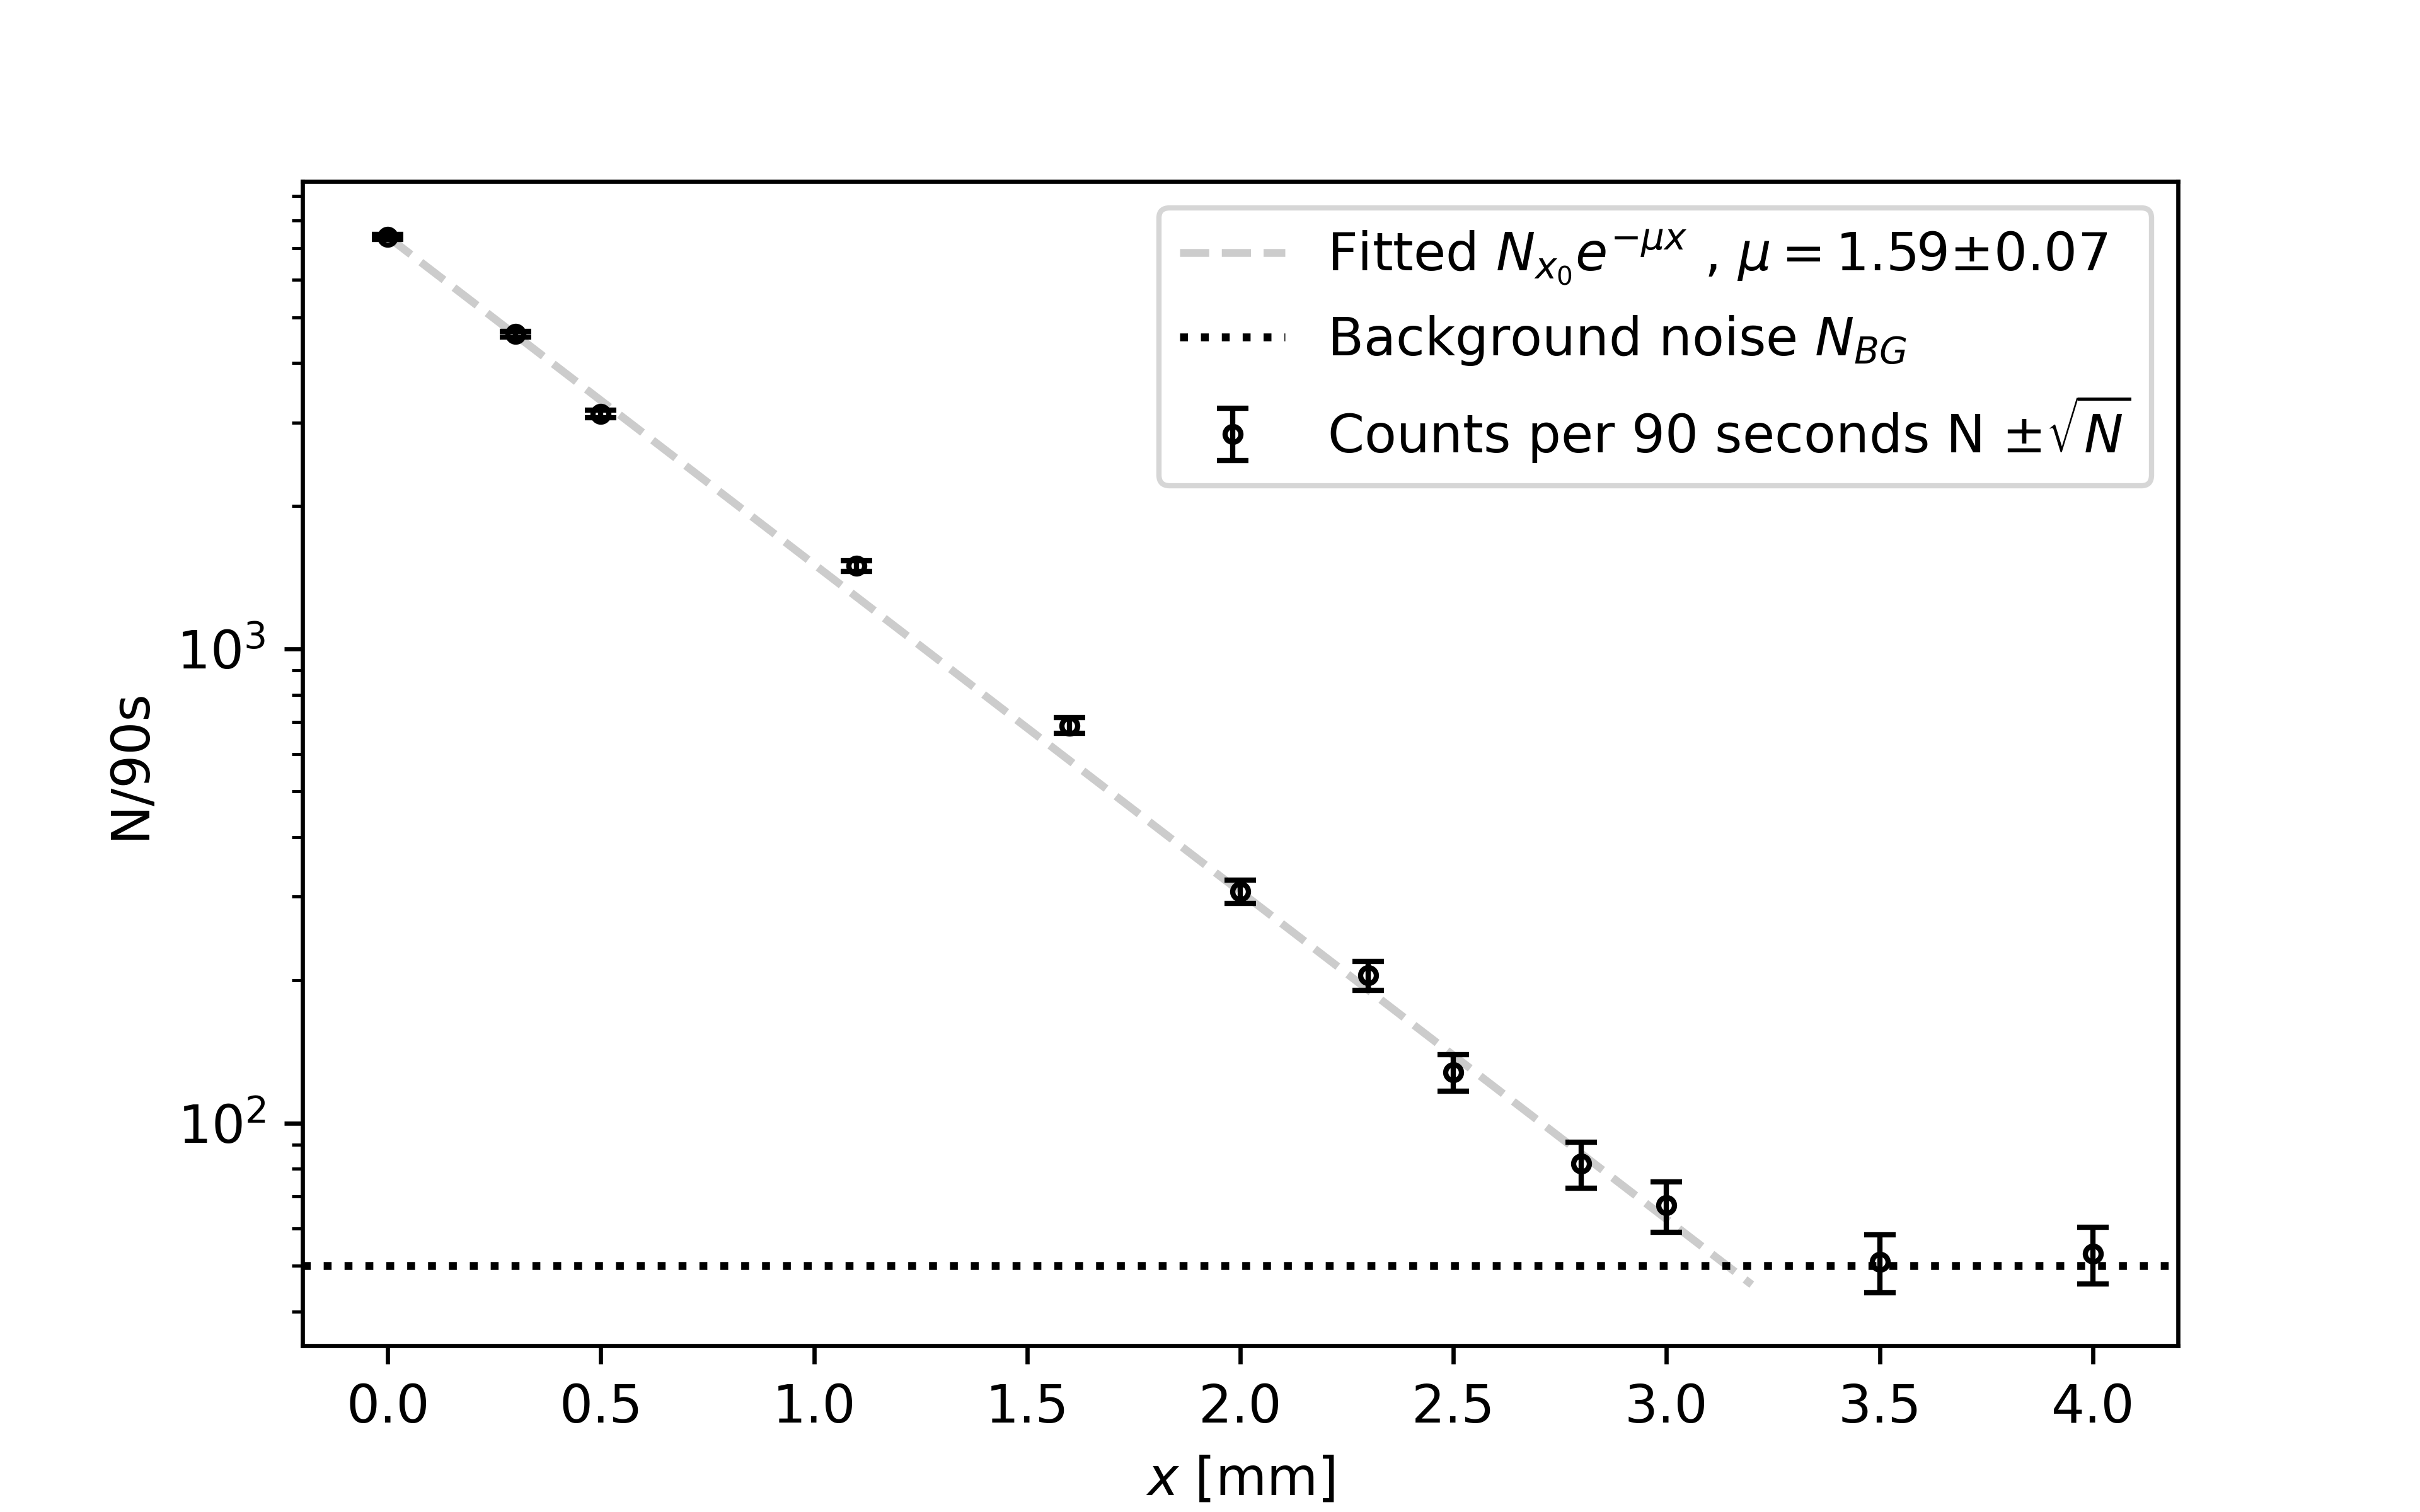
\includegraphics[width=400pt]{python/fit.PNG}
	\caption{Number of counts per \SI{90}{\second} is logarithmically plotted against the thickness of the aluminium plates [\si{\mm}]. The uncertainty of the counted numbers is displayed as error bars on the measured counts.}
	\label{fig::absorb}
\end{figure}